\documentclass[10pt, aspectratio=169]{beamer}

% --- PAQUETES ---
\usepackage[utf8]{inputenc}
\usepackage[spanish]{babel}
\usepackage{amsmath}
\usepackage{amsfonts}
\usepackage{xcolor}
\usepackage{tikz}

% --- CONFIGURACIÓN DE DISEÑO PROFESIONAL (LIENZO TRANSPARENTE) ---
\usetheme{default}
\setbeamercolor{background canvas}{bg=}
\setbeamertemplate{navigation symbols}{}
\setbeamertemplate{headline}{}
\setbeamertemplate{footline}{}

% Colores institucionales
\definecolor{unemiAzul}{RGB}{20,40,90}
\definecolor{unemiNaranja}{RGB}{255,102,0}

% Tipografía
\setbeamerfont{frametitle}{size=\Large, series=\bfseries}
\setbeamercolor{frametitle}{fg=unemiAzul}

% --- FONDO DE LA PRESENTACIÓN ---
\setbeamertemplate{background}{
	\begin{tikzpicture}[remember picture, overlay]
		\node[inner sep=0pt] at (current page.center) {
			
\includegraphics[width=\paperwidth, height=\paperheight]{portadaUNEMI2}
		};
	\end{tikzpicture}
}

\begin{document}
	
	% --- PORTADA ---
	{
		\setbeamertemplate{background}{
\includegraphics[width=\paperwidth, height=\paperheight]{portadaUNEMI}}
		\begin{frame}[plain]
			\begin{tikzpicture}[remember picture, overlay]
				\node[fill=unemiAzul, fill opacity=0.8, text opacity=1, rounded corners, inner sep=20pt] at (current page.center) {
					\begin{minipage}{0.7\textwidth}
						\centering
						{\Huge \textbf{\textcolor{white}{Software y Redes}}} \\
						\vspace{0.4cm}
						{\Large \textcolor{white}{Fundamentos de Tecnologías de la Información}} \\
						\vspace{1cm}
						{\small \textcolor{white}{Estudiante:}} \\
						\textbf{\textcolor{unemiNaranja}{Angel Fernando Calero Maldonado}} \\
						\vspace{0.3cm}
						{\small \textcolor{white}{Universidad Estatal de Milagro}}
					\end{minipage}
				};
			\end{tikzpicture}
		\end{frame}
	}
	
	% --- DIAPOSITIVA 1 ---
	\begin{frame}{Introducción}
		\small
		\begin{block}{}
			Un sistema de cómputo no funciona únicamente por sus componentes físicos. Necesita instrucciones, programas y comunicación entre dispositivos.
		\end{block}
		
		\vspace{0.3cm}
		\begin{itemize}
			\item El \textbf{software} permite que el hardware realice tareas útiles.
			\item Las \textbf{redes} permiten que varios dispositivos compartan información, servicios y recursos.
			\item Ambos elementos son esenciales para el funcionamiento de computadoras, teléfonos, servidores y plataformas digitales.
		\end{itemize}
	\end{frame}
	
	% --- DIAPOSITIVA 2 ---
	\begin{frame}{¿Qué es el Software?}
		
		\vspace{0.35cm}
	
	\makebox[0pt][l]{%
		\hspace*{-1.15cm}
		
		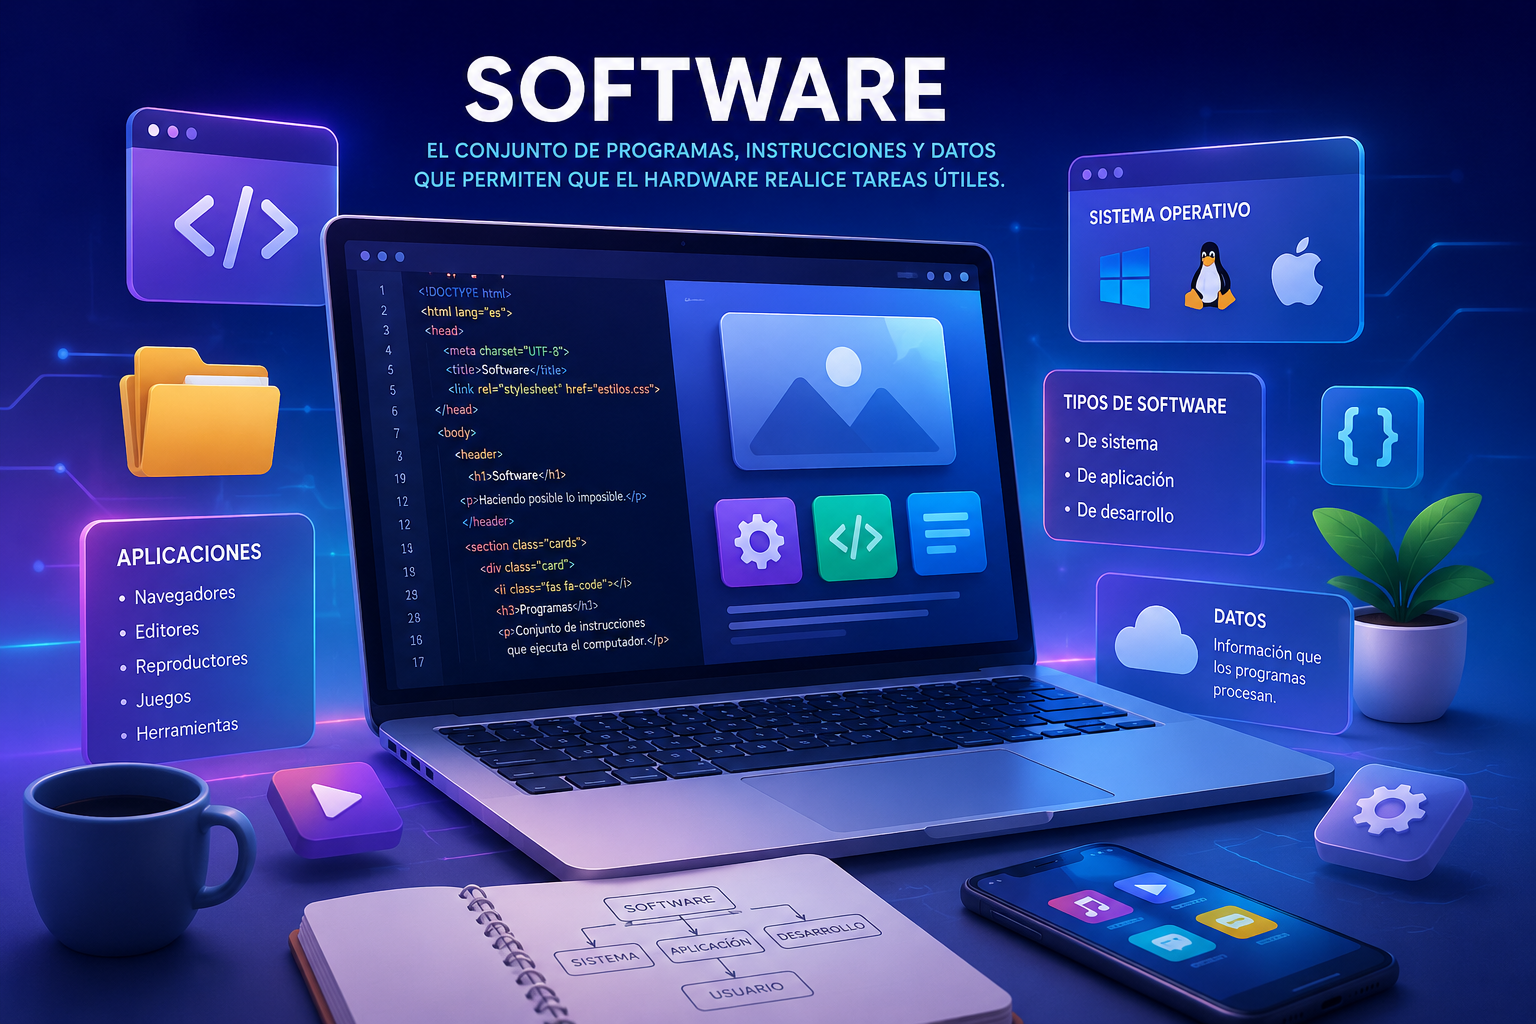
\includegraphics[
		width=\paperwidth,
		height=0.76\paperheight
			]{imagenes/software.png}
			
		}
		
	\end{frame}
	
	% --- DIAPOSITIVA 3 ---
	\begin{frame}{Relación entre Software y Hardware}
			\vspace{0.35cm}
		
		\makebox[0pt][l]{%
			\hspace*{-1.15cm}
			
			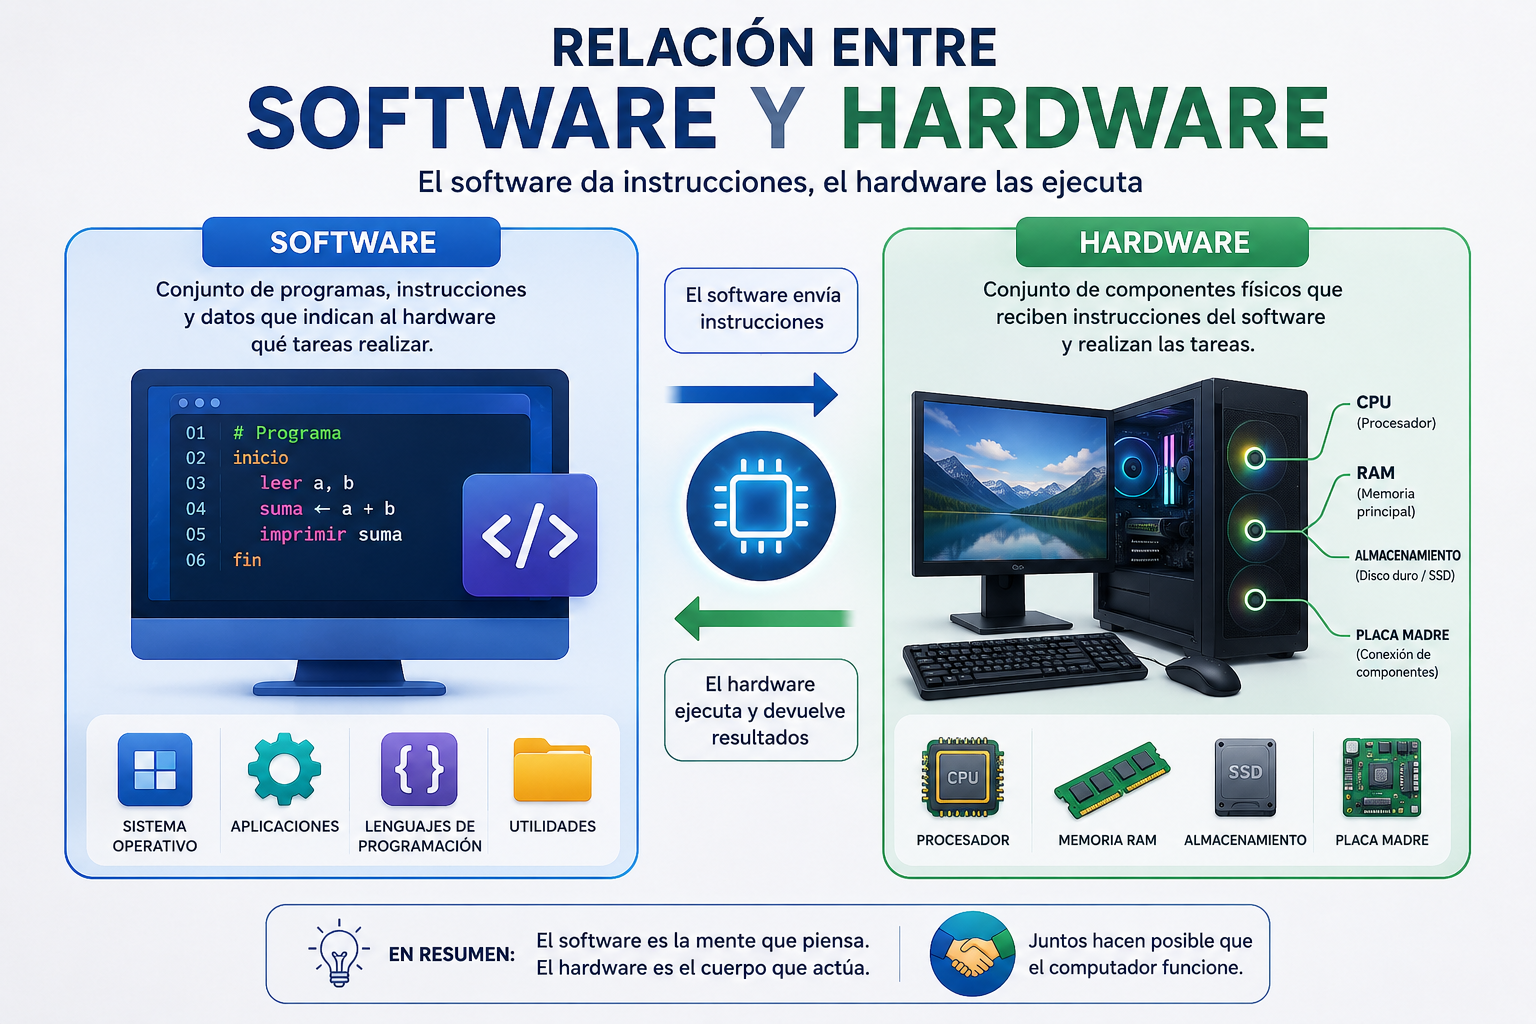
\includegraphics[
			width=\paperwidth,
			height=0.76\paperheight
		]{imagenes/softwareyhardware.png}
		
	}
	\end{frame}
	
	% --- DIAPOSITIVA 4 ---
	\begin{frame}{Tipos Principales de Software}
		\vspace{0.35cm}
	
	\makebox[0pt][l]{%
		\hspace*{-1.15cm}
		
		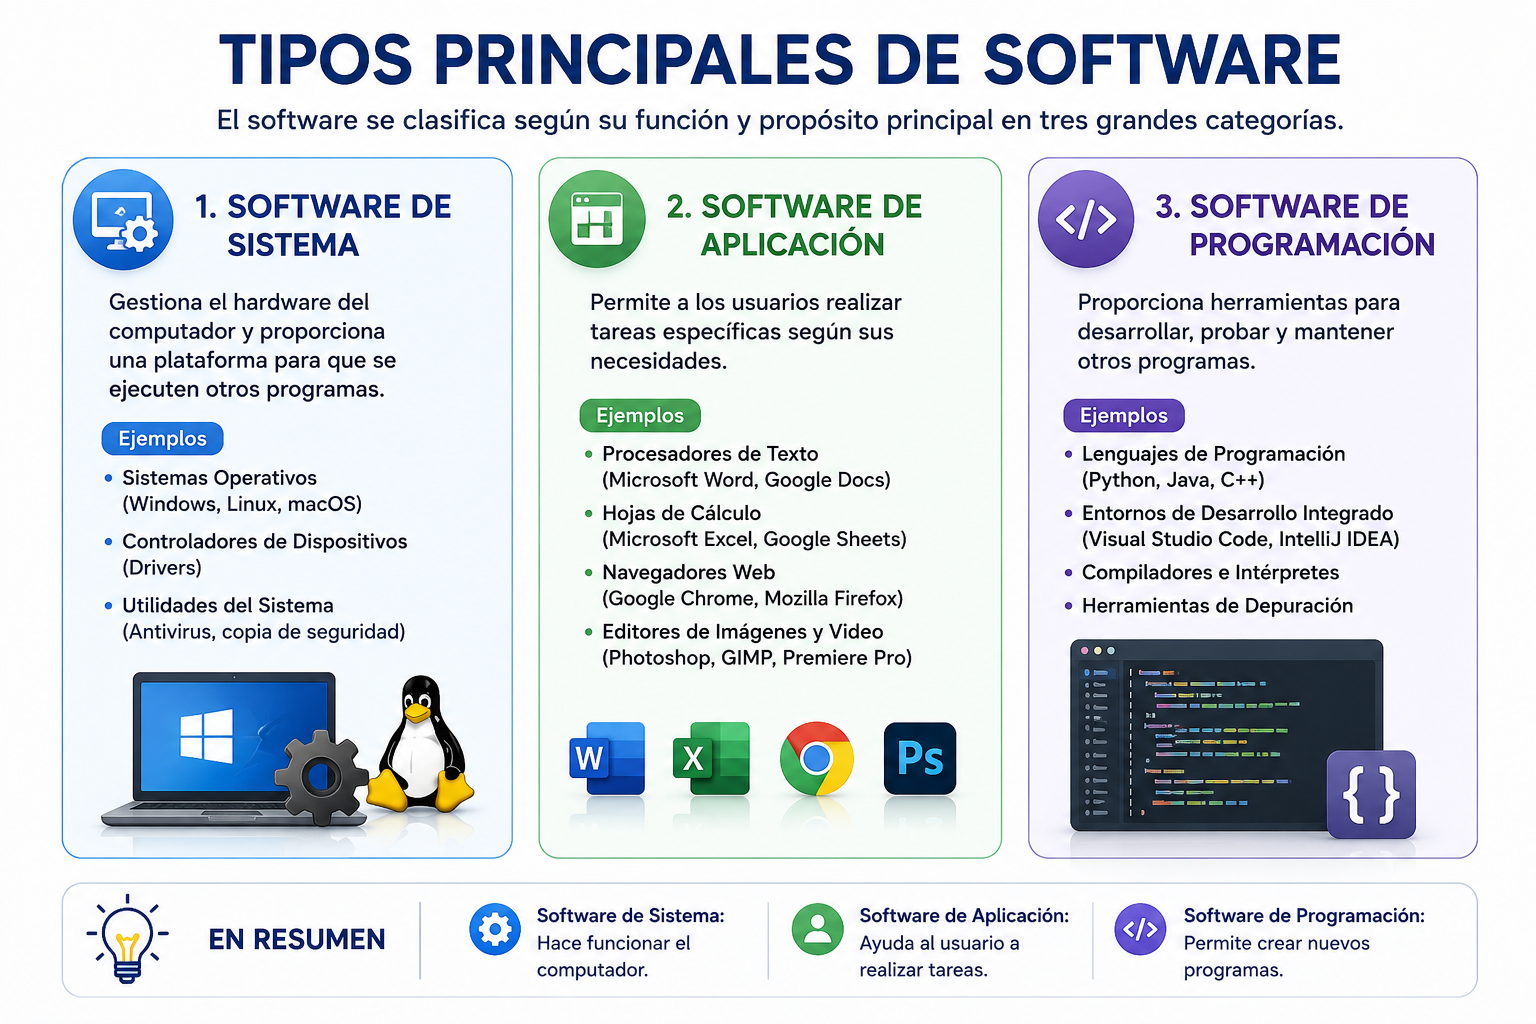
\includegraphics[
		width=\paperwidth,
		height=0.76\paperheight
		]{imagenes/tiposdesoftware.png}
		
	}
	\end{frame}
	


	
	% --- DIAPOSITIVA 9 ---
	\begin{frame}{Importancia del Software}
		\small
		\begin{block}{Importancia}
			El software transforma la capacidad física del computador en soluciones reales para los usuarios.
		\end{block}
		
		\vspace{0.3cm}
		\begin{itemize}
			\item Automatiza tareas repetitivas.
			\item Mejora la productividad académica y laboral.
			\item Permite el acceso a internet, plataformas educativas y servicios digitales.
			\item Facilita la comunicación, el análisis de datos y la creación de contenido.
			\item Hace posible que el hardware sea útil, flexible y adaptable.
		\end{itemize}
	\end{frame}
	
	% --- DIAPOSITIVA 10 ---
	\begin{frame}{¿Qué es una Red de Computadoras?}
		\vspace{0.35cm}
	
	\makebox[0pt][l]{%
		\hspace*{-1.15cm}
		
		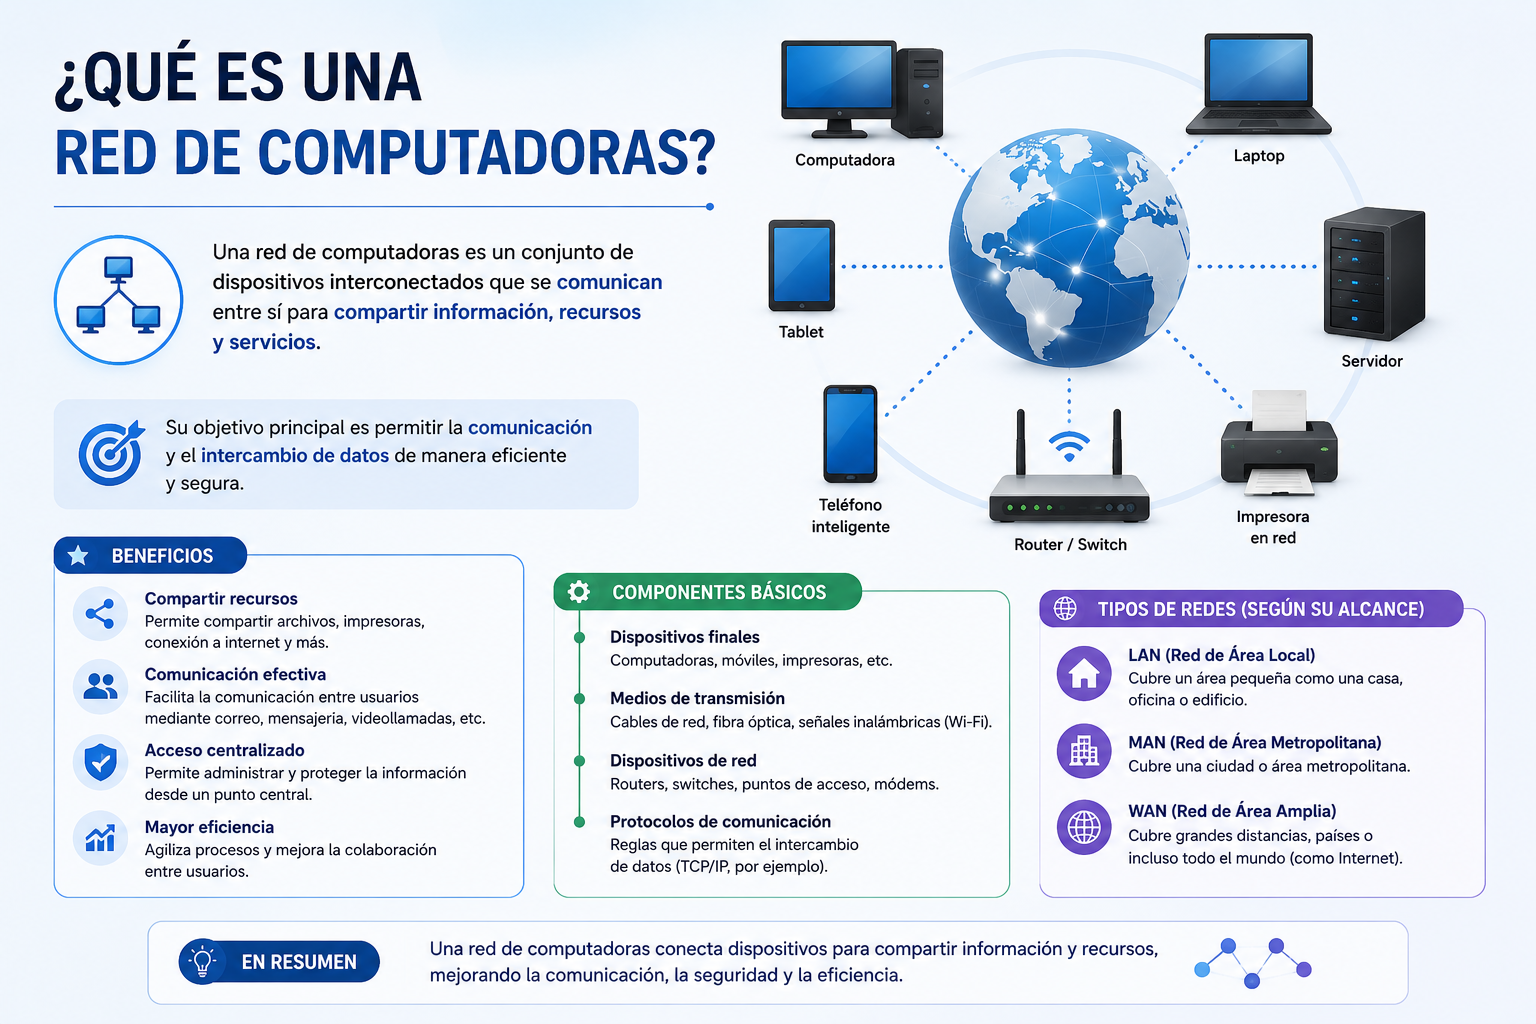
\includegraphics[
		width=\paperwidth,
		height=0.76\paperheight
		]{imagenes/reddecomputadoras.png}
		
	}
	
	\end{frame}
	
% --- DIAPOSITIVA 12 ---
\begin{frame}{Tipos de Redes}
	\vspace{0.35cm}

\makebox[0pt][l]{%
	\hspace*{-1.15cm}
	
	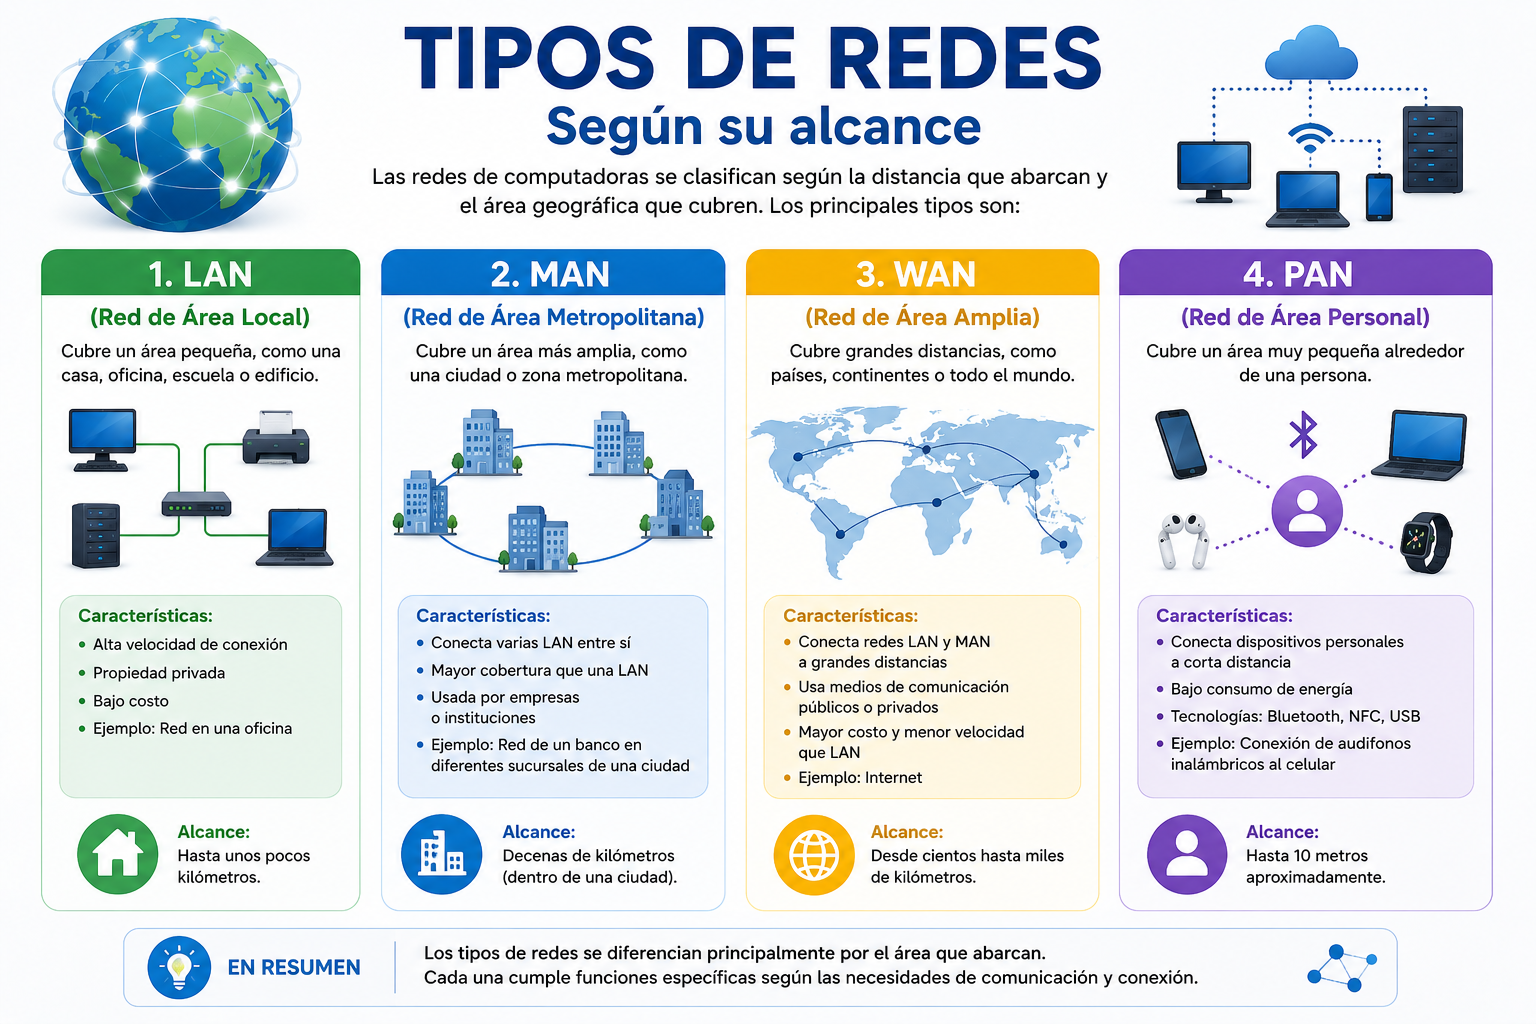
\includegraphics[
	width=\paperwidth,
	height=0.76\paperheight
		]{imagenes/tiposderedes.png}
		
	}
	
\end{frame}
	
	
% --- DIAPOSITIVA 14 ---
\begin{frame}{Elementos Básicos de una Red}
	
	\vspace{0.35cm}
	
	\makebox[0pt][l]{%
		\hspace*{-1.15cm}
		
		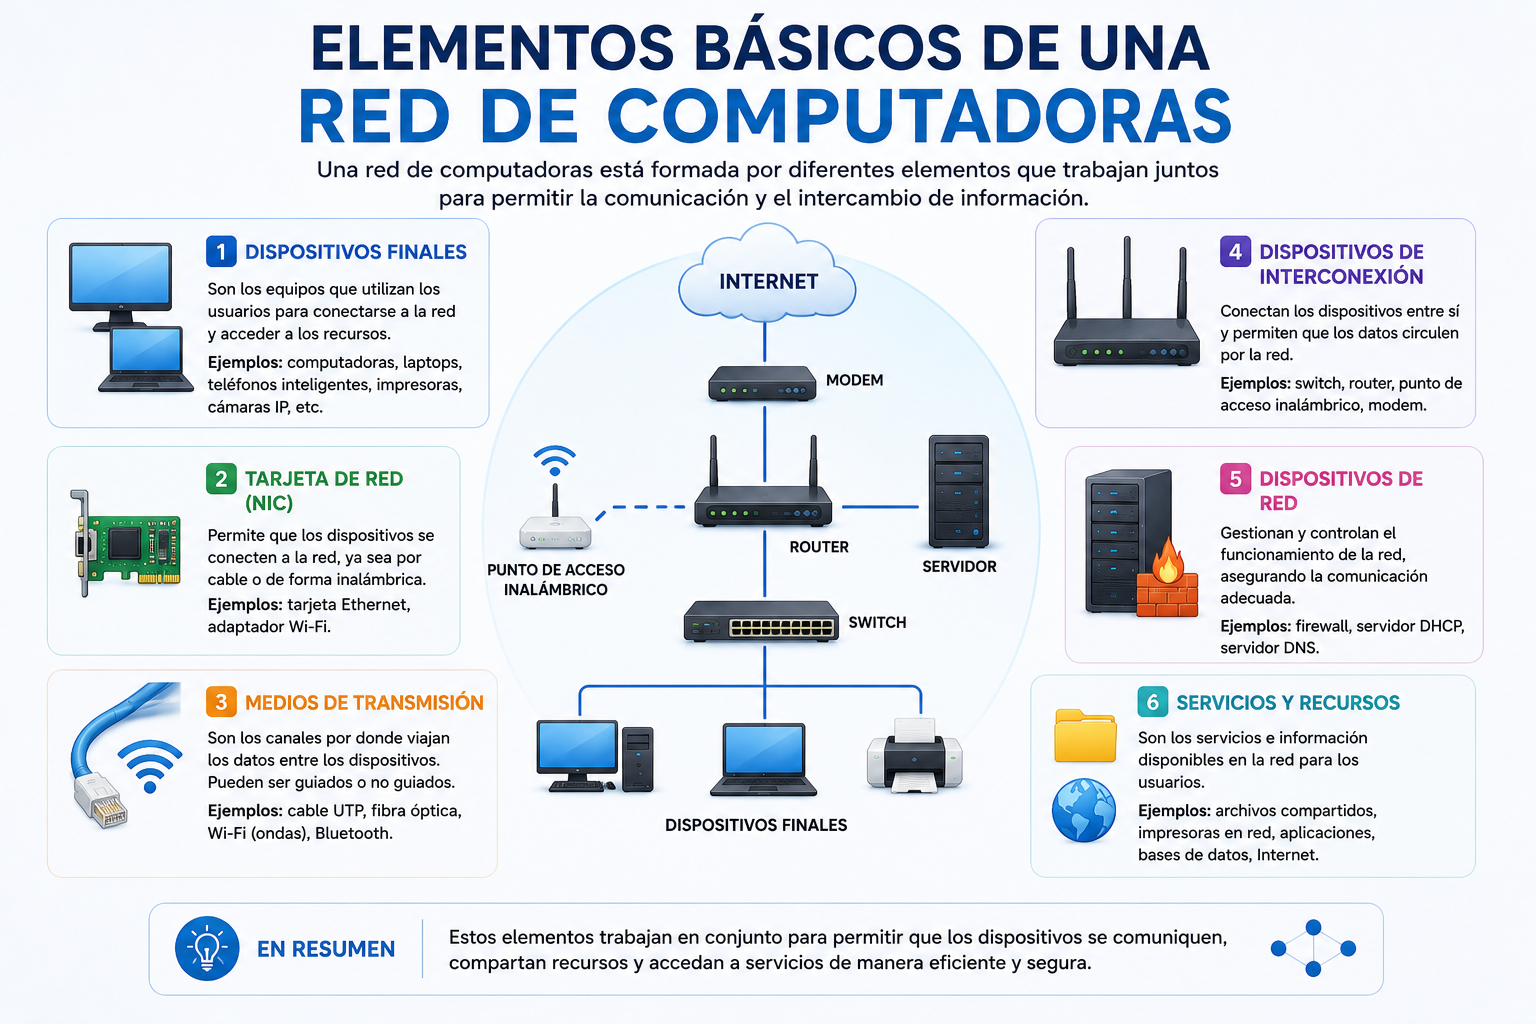
\includegraphics[
		width=\paperwidth,
		height=0.76\paperheight
		]{imagenes/elementosbasicosdeunared.png}
		
	}
	
\end{frame}
	
	% --- DIAPOSITIVA 16 ---
\begin{frame}{Direcciones IP}
	
	\vspace{0.35cm}

    \makebox[0pt][l]{%
		\hspace*{-1.15cm}
	
		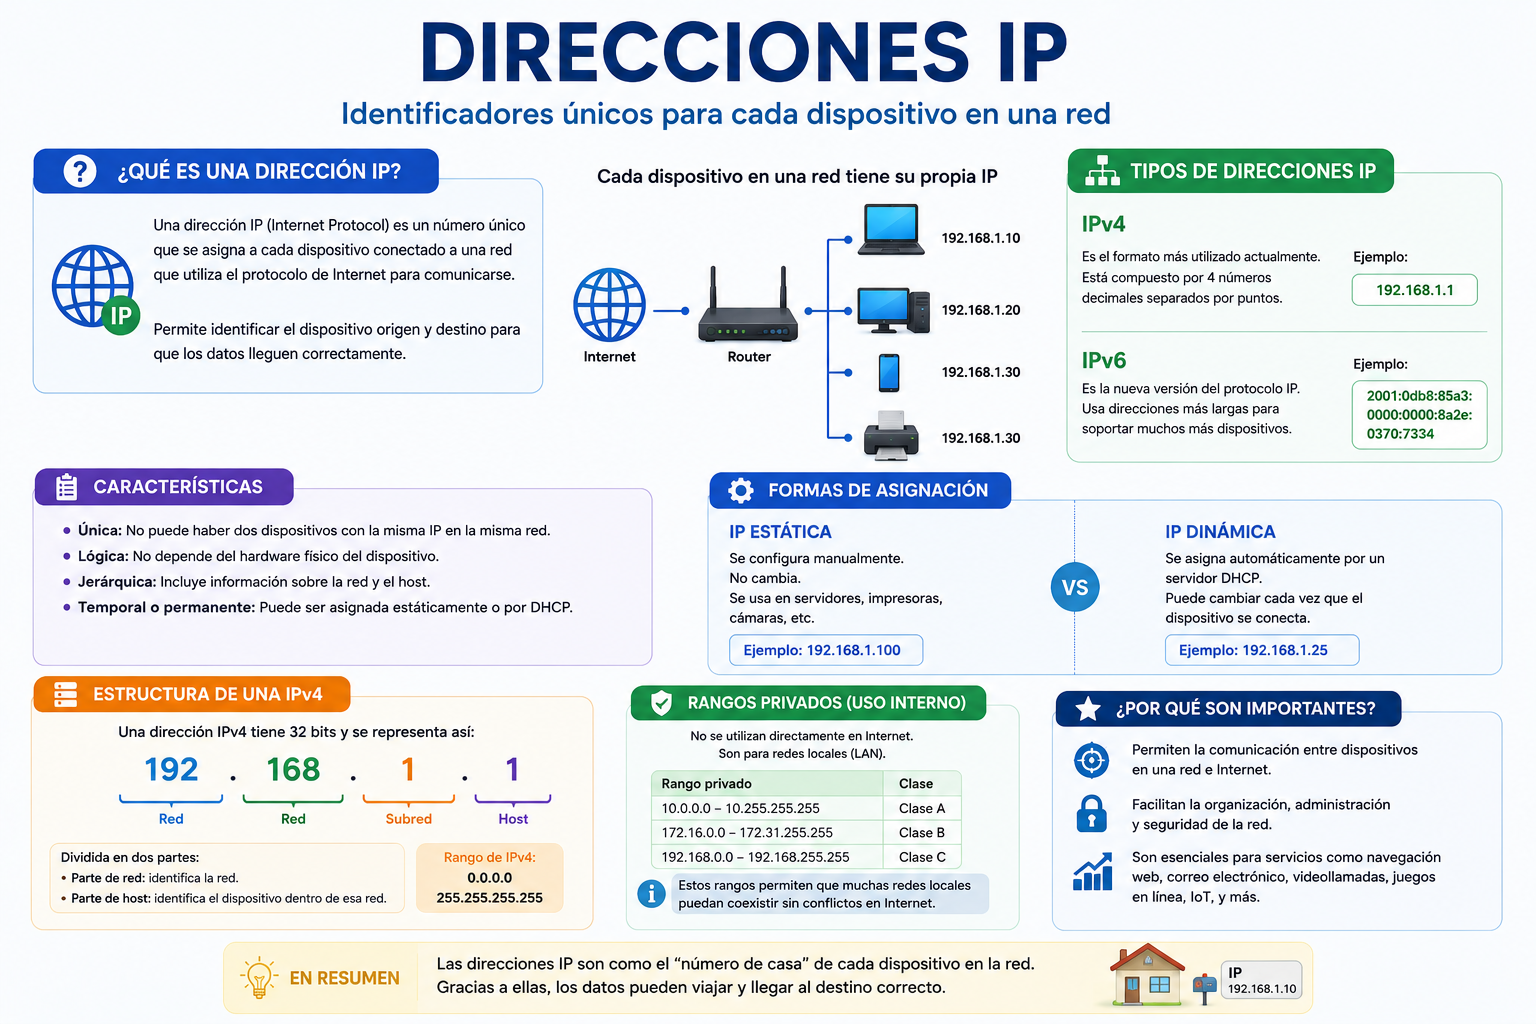
\includegraphics[
		width=\paperwidth,
		height=0.76\paperheight
		]{imagenes/direccionip.png}
	}	
		
\end{frame}
	
	% --- DIAPOSITIVA 17 ---
	\begin{frame}{¿Cómo se Comunican los Dispositivos?}
		\small
		\begin{block}{Proceso general}
			Cuando un dispositivo envía información, los datos se dividen, se identifican, viajan por la red y se reconstruyen en el destino.
		\end{block}
		
		\vspace{0.3cm}
		\begin{itemize}
			\item El mensaje se transforma en datos digitales.
			\item Los datos se dividen en paquetes.
			\item Cada paquete contiene información de origen y destino.
			\item Los dispositivos de red encaminan los paquetes.
			\item El equipo receptor reúne los datos y muestra el resultado.
		\end{itemize}
	\end{frame}
	
	% --- DIAPOSITIVA 18 ---
	\begin{frame}{Protocolos de Comunicación}
		\small
		\begin{block}{Definición}
			Los protocolos son reglas que permiten que los dispositivos se entiendan durante el intercambio de información.
		\end{block}
		
		\vspace{0.3cm}
		\begin{itemize}
			\item \textbf{IP:} identifica y direcciona los paquetes.
			\item \textbf{TCP:} ayuda a que la información llegue completa y ordenada.
			\item \textbf{HTTP/HTTPS:} permite acceder a páginas web.
			\item \textbf{DNS:} traduce nombres de sitios web en direcciones IP.
		\end{itemize}
	\end{frame}
	
	% --- DIAPOSITIVA 19 ---
	\begin{frame}{Seguridad en Software y Redes}
		\small
		\begin{block}{Importancia}
			La seguridad protege la información, los dispositivos y la continuidad de los servicios digitales.
		\end{block}
		
		\vspace{0.3cm}
		\begin{itemize}
			\item Mantener el software actualizado reduce vulnerabilidades.
			\item Usar contraseñas seguras protege el acceso a cuentas y equipos.
			\item Los antivirus y cortafuegos ayudan a detectar amenazas.
			\item El cifrado protege datos durante la transmisión.
			\item Las copias de seguridad permiten recuperar información ante fallos.
		\end{itemize}
	\end{frame}
	
	% --- DIAPOSITIVA 20 ---
	\begin{frame}{Conclusiones}
		\small
		\begin{block}{Síntesis}
			El software y las redes son dos pilares fundamentales de los sistemas de cómputo modernos.
		\end{block}
		
		\vspace{0.3cm}
		\begin{itemize}
			\item El software convierte al hardware en una herramienta útil.
			\item El sistema operativo coordina recursos y permite ejecutar aplicaciones.
			\item Las redes conectan dispositivos para compartir información y servicios.
			\item LAN y WAN se diferencian principalmente por su alcance geográfico.
			\item La comunicación digital depende de dispositivos, direcciones IP y protocolos.
		\end{itemize}
	\end{frame}
	
	% --- DIAPOSITIVA 21 ---
	\begin{frame}{Referencias}
		\scriptsize
		\begin{itemize}
			\item Silberschatz, A., Galvin, P. B., \& Gagne, G. \textit{Operating System Concepts}.
			\item Tanenbaum, A. S., \& Bos, H. \textit{Modern Operating Systems}.
			\item Tanenbaum, A. S., \& Wetherall, D. J. \textit{Computer Networks}.
			\item Kurose, J. F., \& Ross, K. W. \textit{Computer Networking: A Top-Down Approach}.
			\item Stallings, W. \textit{Data and Computer Communications}.
			\item Microsoft Learn. Documentación sobre sistemas operativos y redes.
			\item Cisco Networking Academy. Material introductorio sobre redes de computadoras.
		\end{itemize}
	\end{frame}
	
	% --- DIAPOSITIVA FINAL ---
	{
		\setbeamertemplate{background}{
\includegraphics[width=\paperwidth, height=\paperheight]{portadaUNEMI}}
		\begin{frame}[plain]
			\begin{tikzpicture}[remember picture, overlay]
				\node[fill=unemiAzul, fill opacity=0.8, text opacity=1, rounded corners, inner sep=20pt] at (current page.center) {
					\begin{minipage}{0.9\textwidth}
						\centering
						{\Huge \textbf{\textcolor{white}{Gracias}}} \\
					\end{minipage}
				};
			\end{tikzpicture}
		\end{frame}
	}
	
	
\end{document}